\section{Method}
\label{sec:method}

\begin{figure}[t]
    \centering
    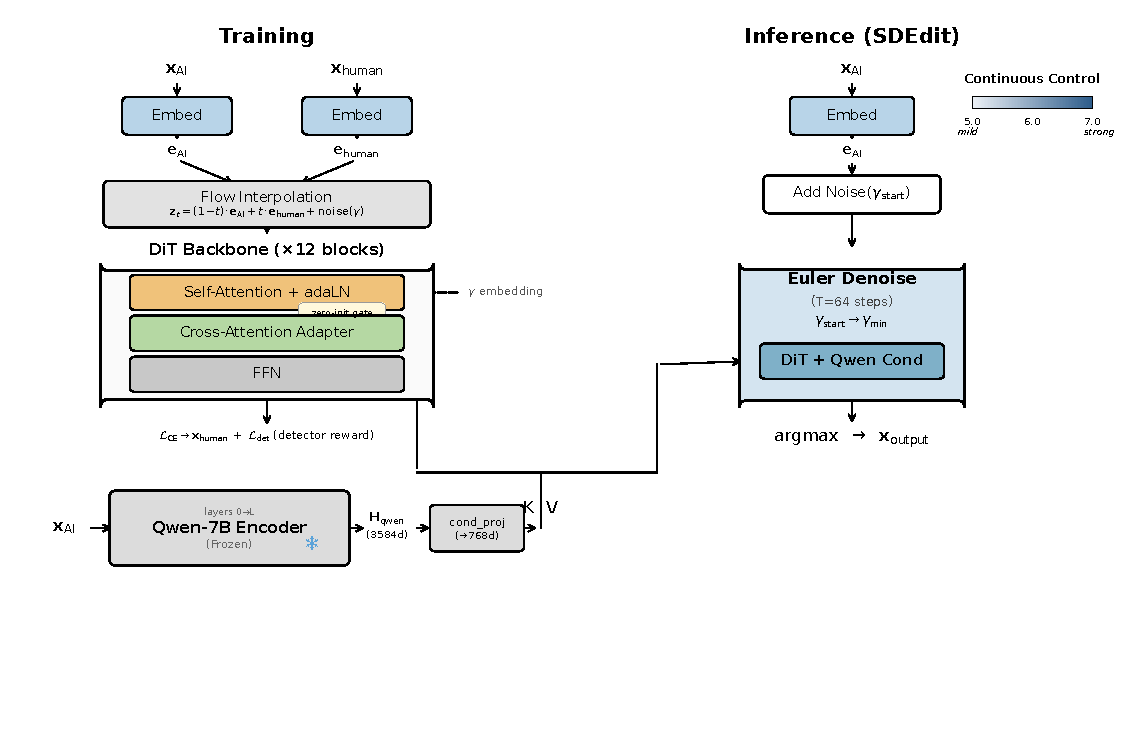
\includegraphics[width=\columnwidth]{figures/fig1_architecture.pdf}
    \caption{Overview of \styleshield{}.
    A pretrained DiT backbone (left) is augmented with zero-initialized
    cross-attention adapters that attend to frozen Qwen-7B hidden
    representations (bottom).
    At inference (right), AI text embeddings are noised at level~$\gamma$
    and iteratively denoised with semantic conditioning via 64 Euler steps.
    The single parameter~$\gamma$ serves as a continuous
    diagnostic axis for characterizing the
    evasion--preservation trade-off.}
    \label{fig:architecture}
\end{figure}

We present \styleshield{}, a conditional flow-matching framework
that operates in continuous token-embedding space, designed as
an adversarial diagnostic for probing AIGC detector robustness.
The system has three components: a DiT backbone pretrained with
flow matching (\S\ref{sec:backbone}), cross-attention adapters
conditioned on a frozen Qwen encoder
(\S\ref{sec:conditioning}), and a training pipeline with
detector-in-the-loop feedback (\S\ref{sec:training}).
At inference a single parameter~$\gamma$ provides continuous
control over transformation intensity, serving as a diagnostic
axis for characterizing detector sensitivity
(\S\ref{sec:inference}).
We further describe \textbf{RateAudit}, a document-level
scheduling algorithm that stress-tests whether detection-rate
verdicts can be set to arbitrary values
(\S\ref{sec:allocator}).
Figure~\ref{fig:architecture} shows the overall architecture.

%% ────────────────────────────────────────────────────
\subsection{Flow Matching Backbone}
\label{sec:backbone}

\styleshield{} operates in continuous token-embedding space via
a Diffusion Transformer
(DiT;~\citealp{peebles2023scalable}) trained with the flow
matching objective~\citep{lipman2023flow, karras2022elucidating}.

\paragraph{Embedding space.}
Each token~$w_i$ is mapped to a $d$-dimensional embedding
$\mathbf{e}_i \in \mathbb{R}^d$ ($d{=}768$) via a learned
vocabulary embedding layer.
Embeddings are length-normalized to stabilize training in the
continuous space:
$\bar{\mathbf{e}} = \sqrt{d}\;\mathbf{e}/\|\mathbf{e}\|$.

\paragraph{Architecture.}
The DiT consists of $N{=}12$ transformer blocks with
self-attention (RoPE), FFN (GELU, expansion ratio~4), and
adaLN-Zero conditioning.
A timestep embedder maps~$\gamma$ to
$\mathbf{c}_\gamma$, which modulates each block:
\begin{equation}
    \mathbf{x}'
      = (1 + \mathbf{s}_\gamma)
        \odot \mathrm{LN}(\mathbf{x})
        + \mathbf{b}_\gamma
\end{equation}
where $\mathbf{s}_\gamma, \mathbf{b}_\gamma$ are predicted from
$\mathbf{c}_\gamma$ via a zero-initialized linear layer.
We additionally employ a bias skip
connection~\citep{karras2022elucidating}:
\begin{equation}
    \mathrm{logits}
      = f_\theta(\mathbf{z},\gamma)
        + c_{\mathrm{skip}}(\gamma)
          \;\mathbf{z}\,\mathbf{W}_{\mathrm{emb}}^\top
\end{equation}
where
$c_{\mathrm{skip}}(\gamma)
  = \exp\bigl((\mathrm{softplus}(-\gamma)-\gamma)/2\bigr)$
provides a direct residual path from the noisy input to the
output logits, stabilizing training at low noise levels.

\paragraph{Noise schedule and Gumbel proposal.}
Following the EDM formulation~\citep{karras2022elucidating},
the forward noising process at noise level~$\gamma$ is:
\begin{equation}
    \mathbf{z}_\gamma
      = \alpha(\gamma)\,\mathbf{x}
      + \sigma(\gamma)\,\boldsymbol{\epsilon},
    \quad
    \boldsymbol{\epsilon}\sim\mathcal{N}(\mathbf{0},\mathbf{I})
    \label{eq:noise}
\end{equation}
where $\alpha(\gamma) = \sqrt{\mathrm{sigmoid}(-\gamma)}$ and
$\sigma(\gamma) = \sqrt{\mathrm{sigmoid}(\gamma)}$.
During training, noise levels are sampled from a learned Gumbel
proposal
$\gamma \sim \mathrm{Gumbel}(\mu, \beta)$.

%% ────────────────────────────────────────────────────
\subsection{Cross-Attention Conditioning}
\label{sec:conditioning}

Style transfer, unlike unconditional generation, must preserve
the semantic content of a \emph{specific} input text.
We inject this content signal via cross-attention adapters
conditioned on a frozen large language model.

\paragraph{Semantic encoder.}
We use Qwen-2.5-7B-Instruct~\citep{qwen2024qwen25} as a frozen
feature extractor.
The AI-text input is tokenized with the Qwen tokenizer and
passed through layers~$0$ to~$L{-}1$
(default $L{=}14$ of 28); the resulting hidden states
$\mathbf{H}_{\mathrm{qwen}}
  \!\in\! \mathbb{R}^{B \times S_q \times 3584}$
encode the semantic content to be preserved.
A learned projection
$\mathrm{proj}\!:\!\mathbb{R}^{3584}{\to}\mathbb{R}^{768}$
maps Qwen features to the DiT hidden dimension.
The Qwen model is kept entirely frozen throughout training---no
gradients flow through it.
The choice of split layer~$L$ trades surface-level fidelity
against semantic abstraction; we ablate
$L\!\in\!\{7,14,21\}$ in \S\ref{sec:ablation}, finding
$L{=}14$ optimal.

\paragraph{Adapter architecture.}
After each DiT self-attention block we insert a
\textbf{cross-attention adapter}.
Each adapter performs multi-head cross-attention where queries
come from the flow tokens and keys/values come from the
projected Qwen hidden states:
\begin{align}
    \mathbf{Q} &= \mathbf{W}_q\;\mathrm{LN}(\mathbf{x}),
    \quad
    [\mathbf{K};\mathbf{V}]
      = \mathbf{W}_{kv}\;\mathrm{proj}(\mathbf{H}_{\mathrm{qwen}})
    \label{eq:cross-kv}\\[2pt]
    \mathbf{x}'
      &= \mathbf{x}
       + \underbrace{g(\mathbf{c}_\gamma)}_{\text{zero-init gate}}
         \!\odot\;
         \mathrm{MHA}(\mathbf{Q},\mathbf{K},\mathbf{V})
    \label{eq:cross-gate}
\end{align}
The gate
$g(\mathbf{c}_\gamma)
  = \mathbf{W}_g\,\mathbf{c}_\gamma + \mathbf{b}_g$
is initialized to zero
($\mathbf{W}_g{=}\mathbf{0},\;\mathbf{b}_g{=}\mathbf{0}$).
This zero initialization is critical: at the start of training,
the adapters have no effect ($g \equiv \mathbf{0}$), so the
model is exactly the pretrained backbone.
The gates gradually open as training progresses, allowing the
model to smoothly learn to incorporate semantic conditioning
without catastrophic forgetting of the pretrained generative
capability.
Each adapter adds $\sim$4$d^2$ parameters per block
($\sim$28M total across 12~blocks), a modest overhead.

%% ────────────────────────────────────────────────────
\subsection{Training}
\label{sec:training}

\paragraph{Data construction.}
We construct 436K parallel (AI, human) text pairs across three
Chinese-language domains---social media (346K), news (68K), and
academic abstracts (22K).
For each domain, we collect human-written texts and prompt
Qwen-2.5-7B-Instruct to rewrite them into AI style.
Each pair is then scored by the AIGC detector and subjected to
\textbf{dual-end strict filtering}: we retain only pairs where
the human side scores $\pai < 0.1$ and the AI side scores
$\pai > 0.9$, ensuring a clean stylistic separation between
the two ends of every training pair.

\paragraph{Denoising objective.}
Given a pair $(x_{\mathrm{AI}}, x_{\mathrm{hu}})$, we embed
both texts, sample $t\!\sim\!\mathcal{U}(0,1)$ and~$\gamma$
from the Gumbel proposal, form the noisy input via flow
interpolation
$\mathbf{z}
  = (1{-}t)\,\mathbf{e}_{\mathrm{AI}}
  + t\,\mathbf{e}_{\mathrm{hu}}$
followed by noise corruption (Eq.~\ref{eq:noise}), and
minimize the denoising cross-entropy:
\begin{equation}
    \mathcal{L}_{\mathrm{CE}}
      = -\!\sum_{i=1}^{S}
          \log\, p_\theta\!\bigl(
            w_i^{\mathrm{hu}}
            \;\big|\;
            \mathbf{z}_\gamma,\; \gamma,\;
            \mathbf{H}_{\mathrm{qwen}}
          \bigr)
    \label{eq:ce}
\end{equation}
The Qwen condition $\mathbf{H}_{\mathrm{qwen}}$ is computed
from~$x_{\mathrm{AI}}$; thus the model learns to denoise
toward the human target while attending to the source semantics.

\paragraph{Detector-in-the-loop reward.}
After a 5{,}000-step warmup we introduce an auxiliary
adversarial signal from a frozen BERT-based AIGC detector.
Periodically, we run inference on a training batch, score the
outputs, and add a reward term:
\begin{equation}
    \mathcal{L}
      = \mathcal{L}_{\mathrm{CE}}
      + \lambda_{\mathrm{det}}\;
        \pai\!\bigl(\hat{x}\bigr),
    \qquad \lambda_{\mathrm{det}} = 0.1
    \label{eq:loss}
\end{equation}
where $\pai(\hat{x})$ is the detector's confidence that the
generated text~$\hat{x}$ is AI-written.
Rather than simply maximizing evasion, this signal acts as a
\emph{quality regularizer}: it encourages the model to achieve
evasion through targeted stylistic shifts rather than content
distortion, yielding lower perplexity at comparable evasion
rates (see A2 ablation, \S\ref{sec:ablation}).

%% ────────────────────────────────────────────────────
\subsection{SDEdit Inference}
\label{sec:inference}

At test time we adapt the SDEdit paradigm~\citep{meng2022sdedit}
to token embeddings:
(1)~embed the input AI text to obtain
$\mathbf{e}_{\mathrm{AI}}$ and extract Qwen condition
$\mathrm{cond\_kv}$;
(2)~corrupt at level $\gamma_{\mathrm{start}}$:
$\mathbf{z}_0
  = \alpha(\gamma_{\mathrm{start}})\,\mathbf{e}_{\mathrm{AI}}
  + \sigma(\gamma_{\mathrm{start}})\,\boldsymbol{\epsilon}$;
(3)~apply $T{=}64$ Euler steps conditioning on
$\mathrm{cond\_kv}$;
(4)~decode via $\arg\max$.
The parameter $\gamma_{\mathrm{start}}$ serves as a
\textbf{continuous diagnostic axis}: low~$\gamma$ yields high
similarity and low evasion; high~$\gamma$ applies stronger
transformation at graceful similarity cost---a capability
fundamentally inaccessible to discrete-token methods.

%% ────────────────────────────────────────────────────
\subsection{RateAudit: Document-Level Scheduling}
\label{sec:allocator}

Deployed AIGC detectors typically process documents in
fixed-length windows ($\leq$512 tokens), then aggregate
window-level scores into a document verdict.
\textbf{RateAudit} exploits this aggregation step to
demonstrate that any pre-specified target detection rate can be
achieved on arbitrarily long texts while preserving semantic
coherence---directly questioning the reliability of
detection-rate-based document verdicts.

Given document~$D$ and a pre-specified target
rate~$r_{\mathrm{target}}$:
\begin{enumerate}\setlength\itemsep{2pt}
    \item \textbf{Segment.}
          Split $D$ into chunks
          $\{c_1, \ldots, c_n\}$ of~$\leq$512 tokens.
    \item \textbf{Score.}
          Compute $\pai(c_i)$ for each chunk;
          aggregate as weighted average
          $\bar{s} = \sum_i w_i\, \pai(c_i)$ with
          $w_i = |c_i|/|D|$.
    \item \textbf{Allocate.}
          Greedily select the highest-$\pai$ chunk and
          rewrite it with \styleshield{} using adaptive~$\gamma$
          ($6.0 \to 6.5 \to 7.0 \to 7.5$), re-scoring after
          each rewrite.
    \item \textbf{Terminate.}
          Stop when
          $\bar{s} \leq r_{\mathrm{target}} + \epsilon$
          ($\epsilon{=}0.02$); an overshoot-skip heuristic
          avoids unnecessary rewrites.
\end{enumerate}
The key empirical insight is that most documents have a small
number of high-$\pai$ ``hot'' chunks; rewriting only these
suffices to shift the aggregate score while leaving the majority
of the document---and its semantic coherence---untouched.

